\section{研究背景和主要工作}

\subsection{研究背景}

\begin{frame}{行人重识别的研究内容}
\begin{block}{}
    行人重识别,指的是在多个视野不重叠的监控视频中,重新识别那些之前出现过的行人,即把当前行人与之前已标记的人物相对应。
\end{block}
\begin{figure}
    \centering
    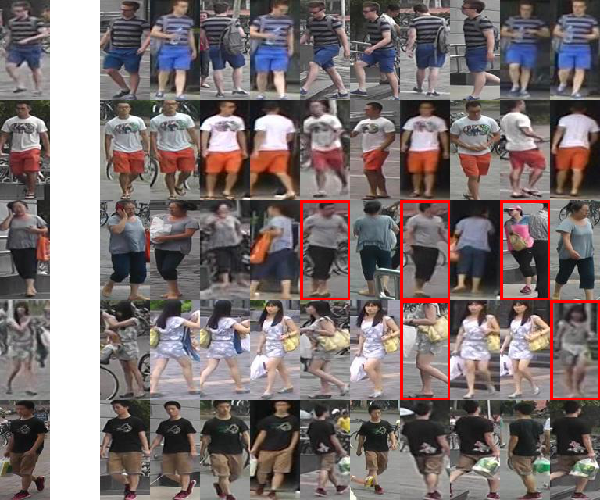
\includegraphics[width=0.6\textwidth,trim={0 200 0 0},clip=true]{figures/vis3}
    \caption{行人重识别解决的问题}
    \label{fig:reid_intro}
\end{figure}
\end{frame}


\begin{frame}{摄像头选择}
\begin{block}{}
    从下图可以看出,相同拍摄地点的不同摄像头所拍摄的画面之间存在较大差异,如角度、光线、拍摄范围与通过时长。这些差异可能会影响行人重识别/跟踪的效果。
\end{block}
\begin{table}
    \centering
    \begin{tabular}{c}
        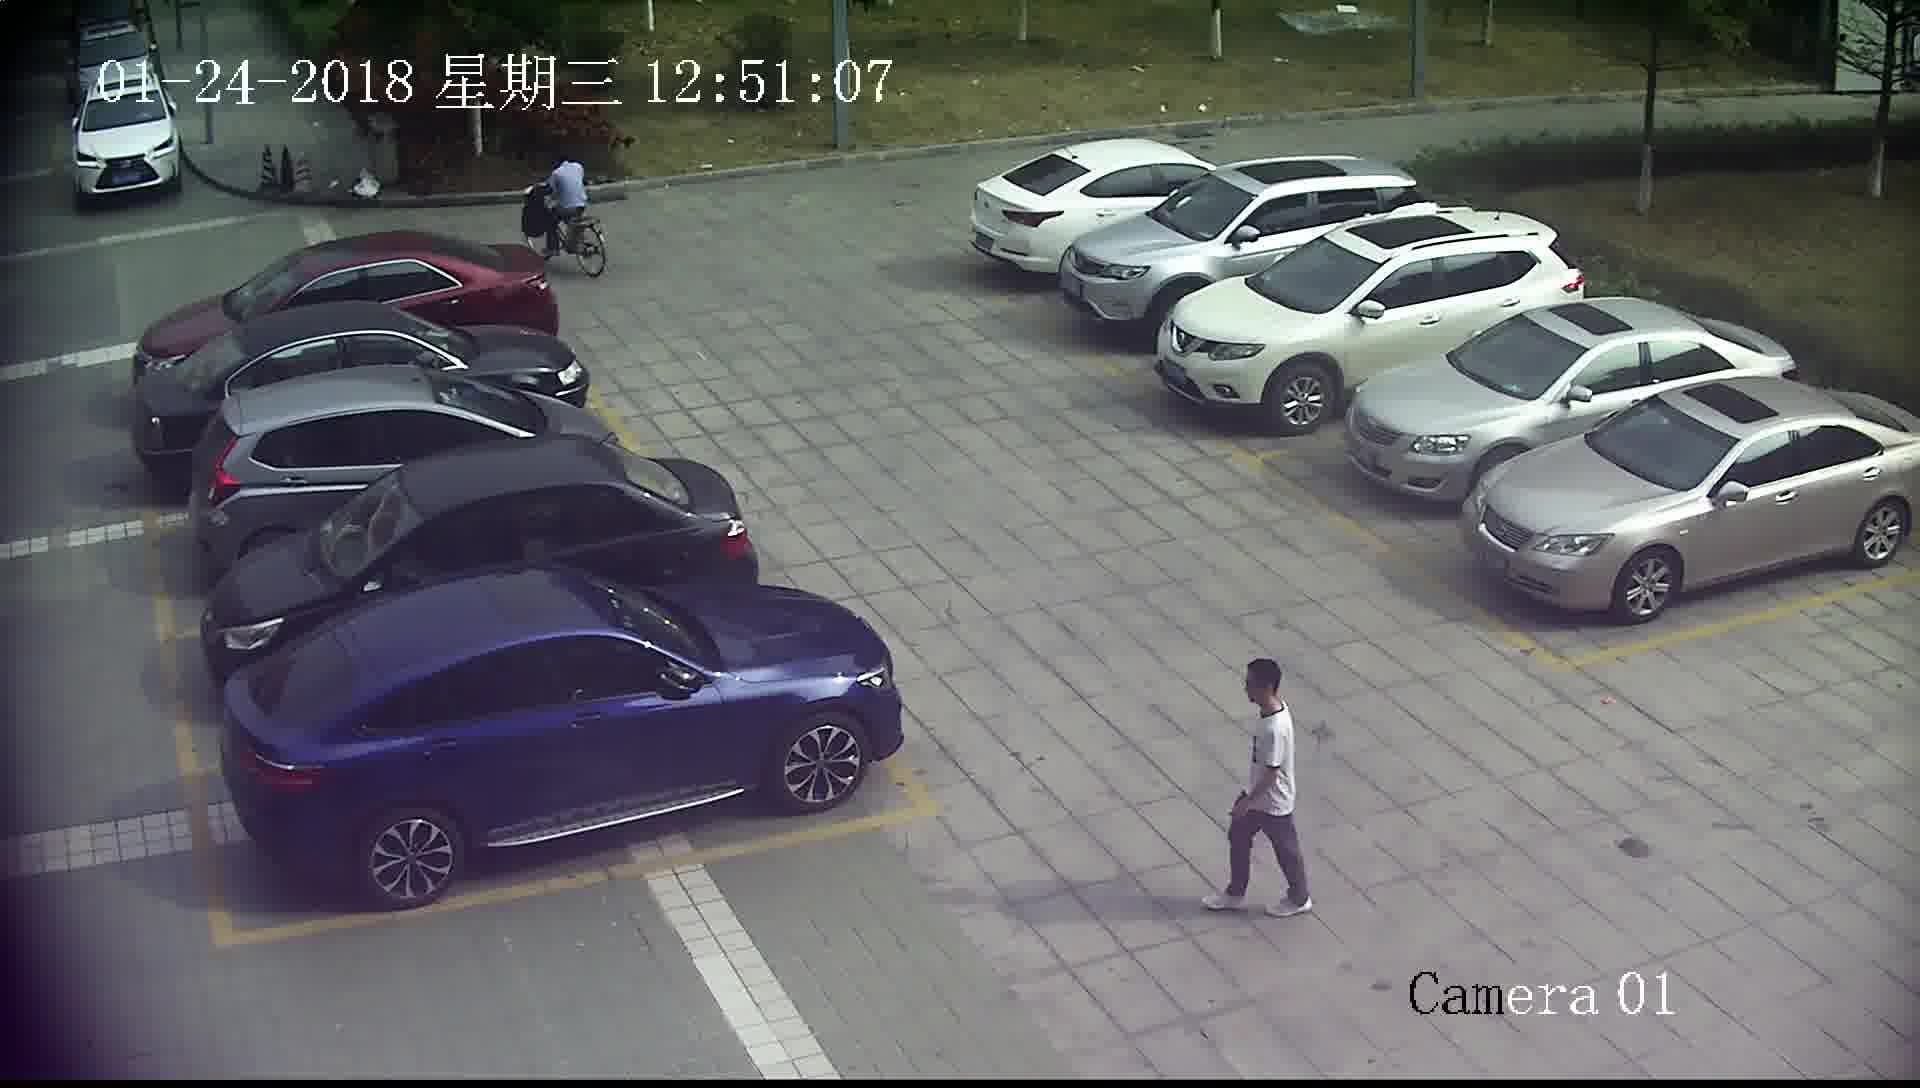
\includegraphics[width=12mm]{figures/1-1}~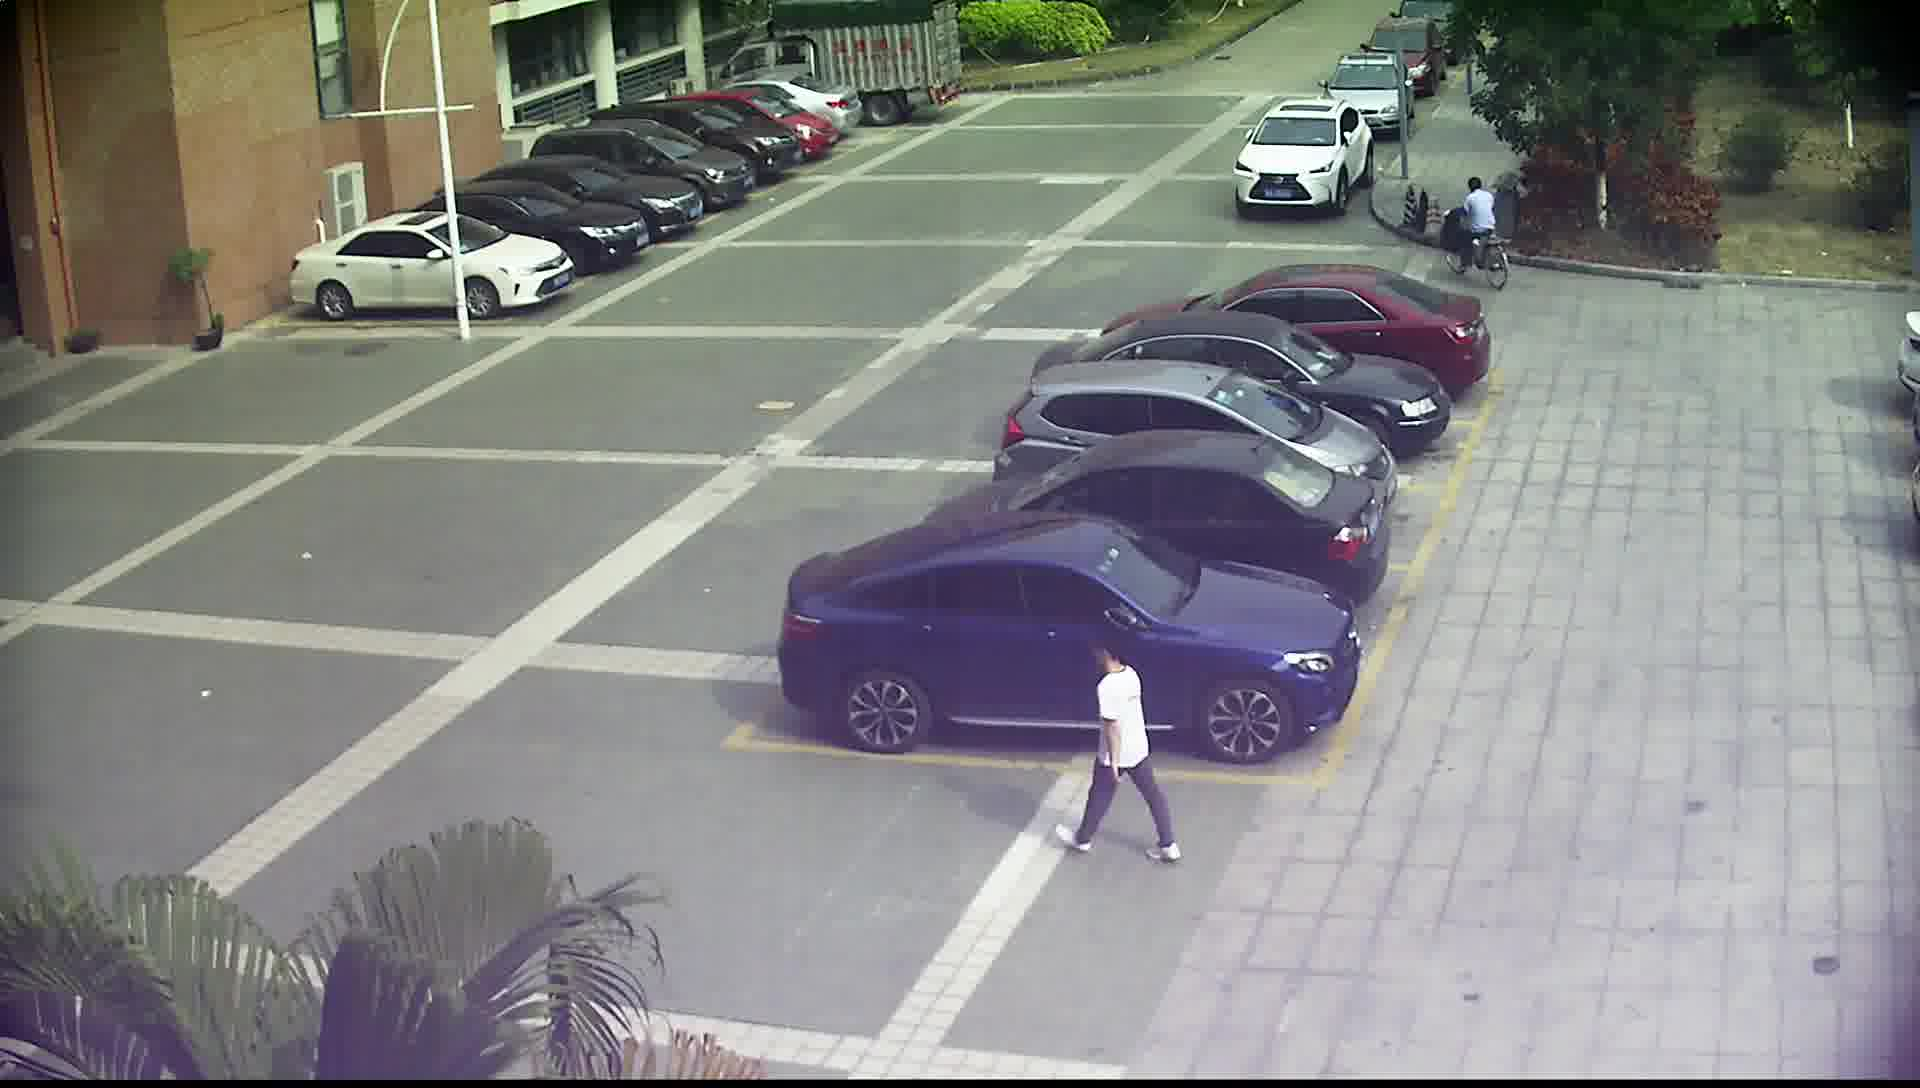
\includegraphics[width=12mm]{figures/1-2} \\
        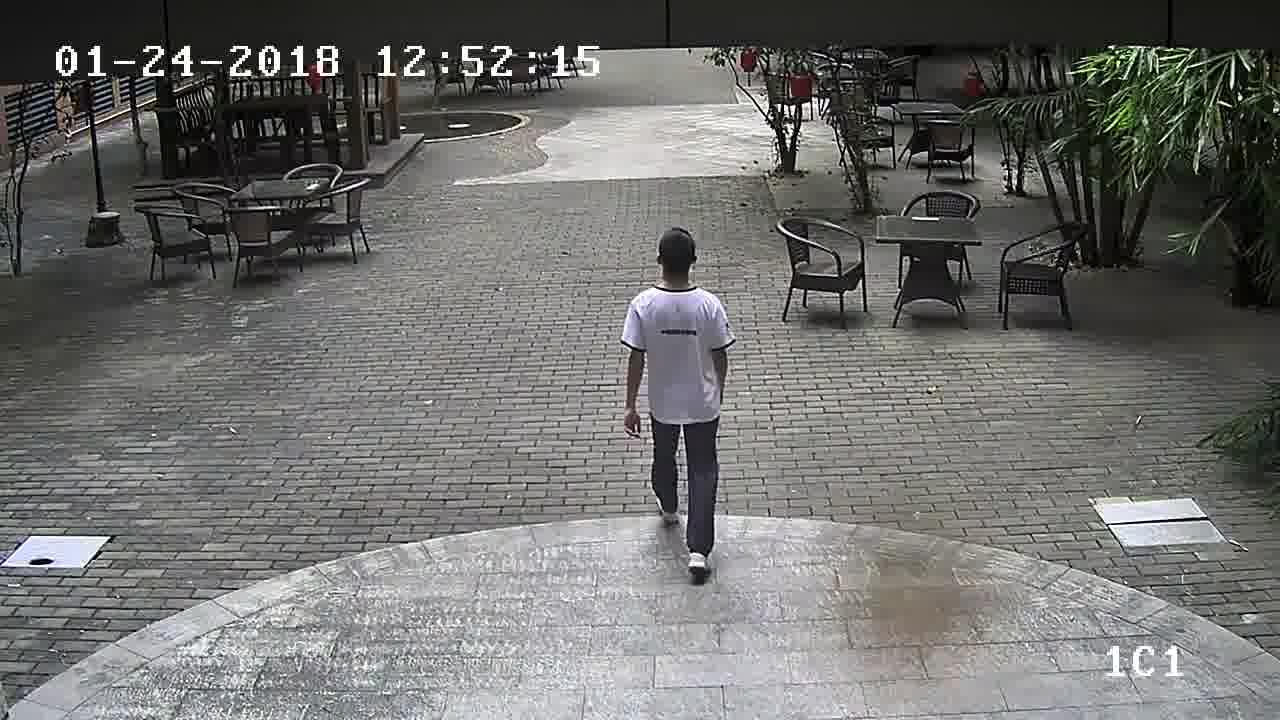
\includegraphics[width=12mm]{figures/1-4}~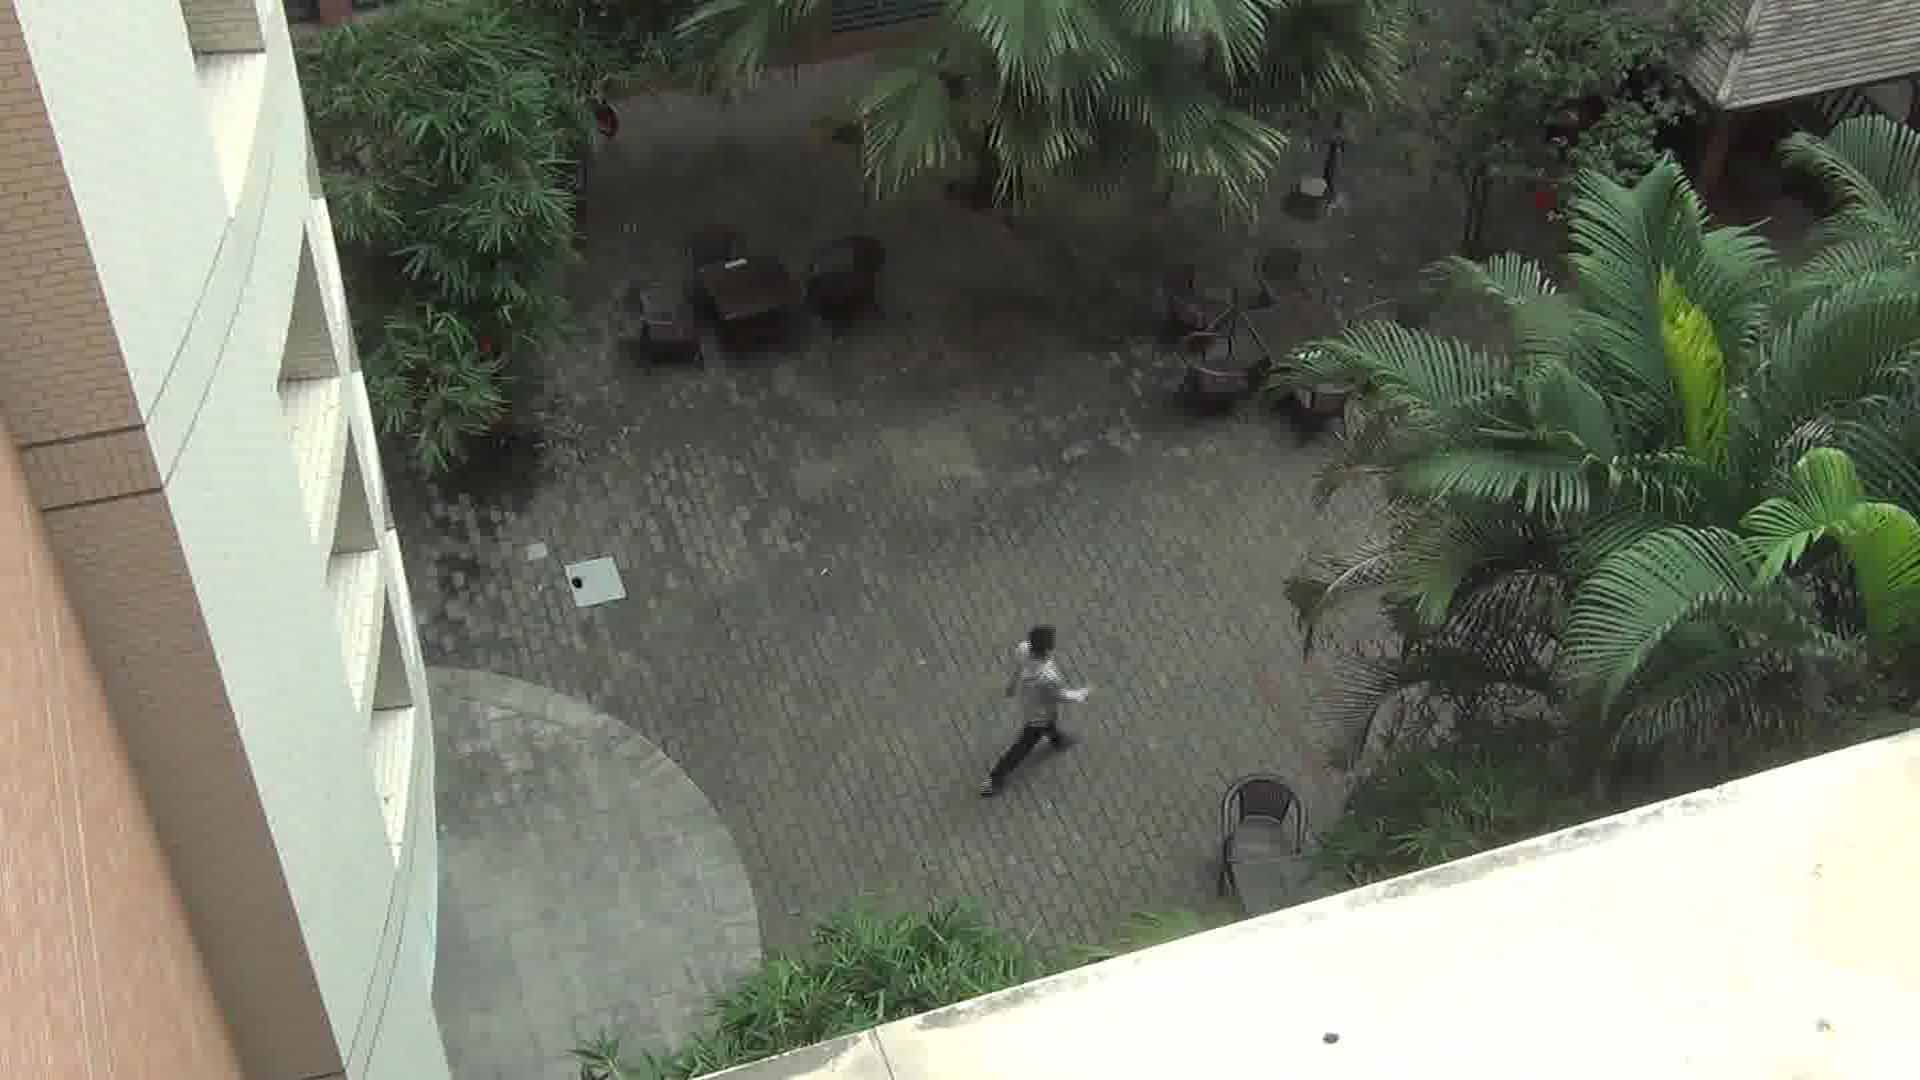
\includegraphics[width=12mm]{figures/1-5}~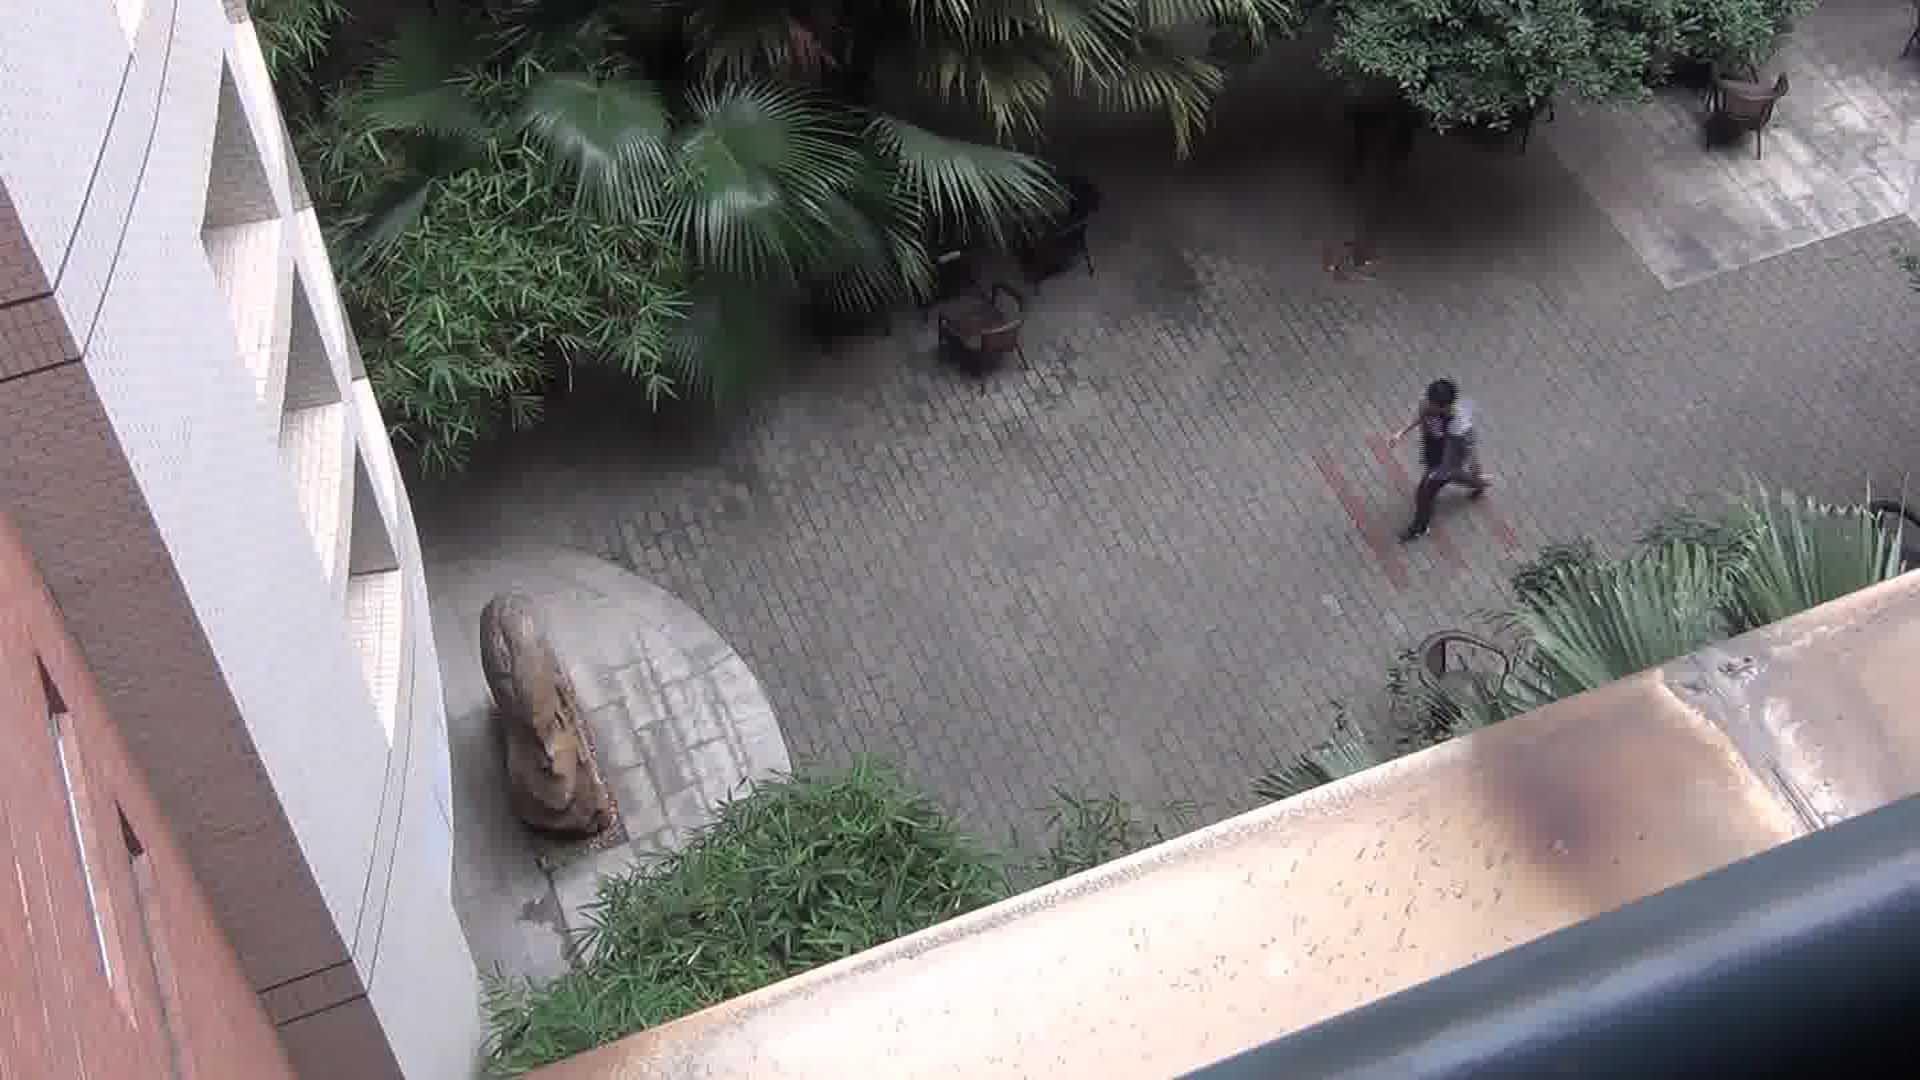
\includegraphics[width=12mm]{figures/1-6} \\
        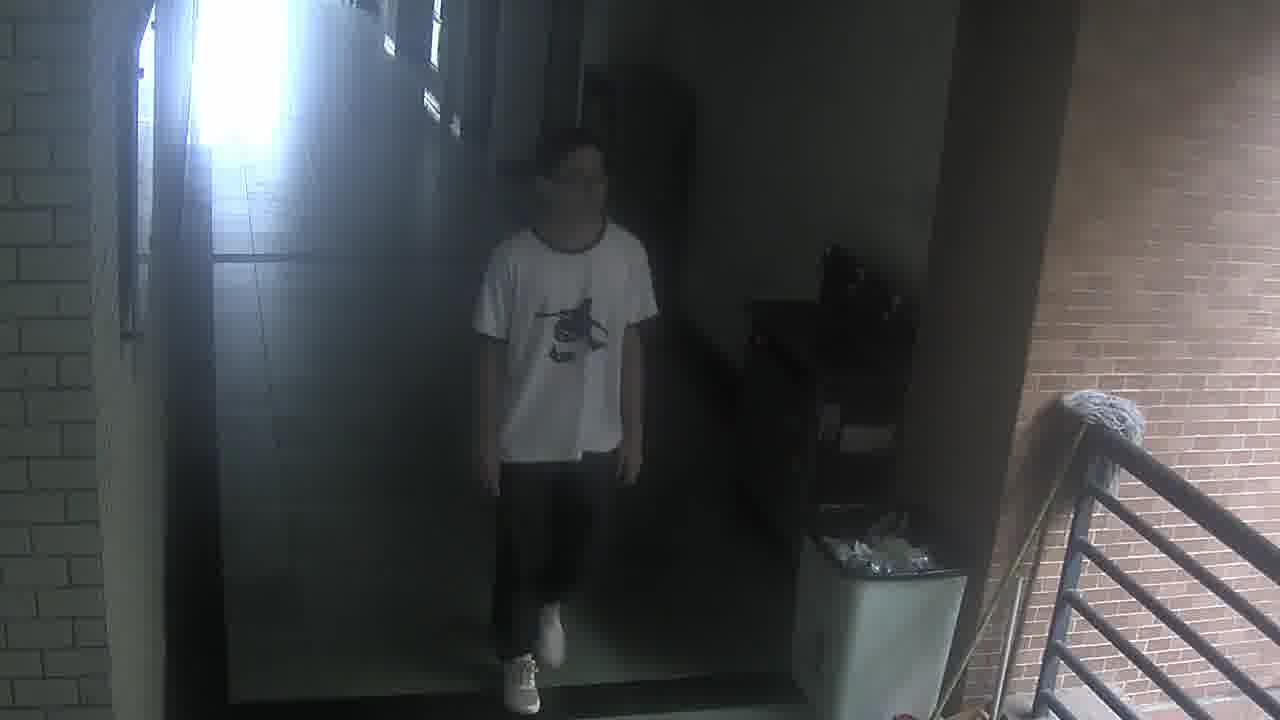
\includegraphics[width=12mm]{figures/2-1}~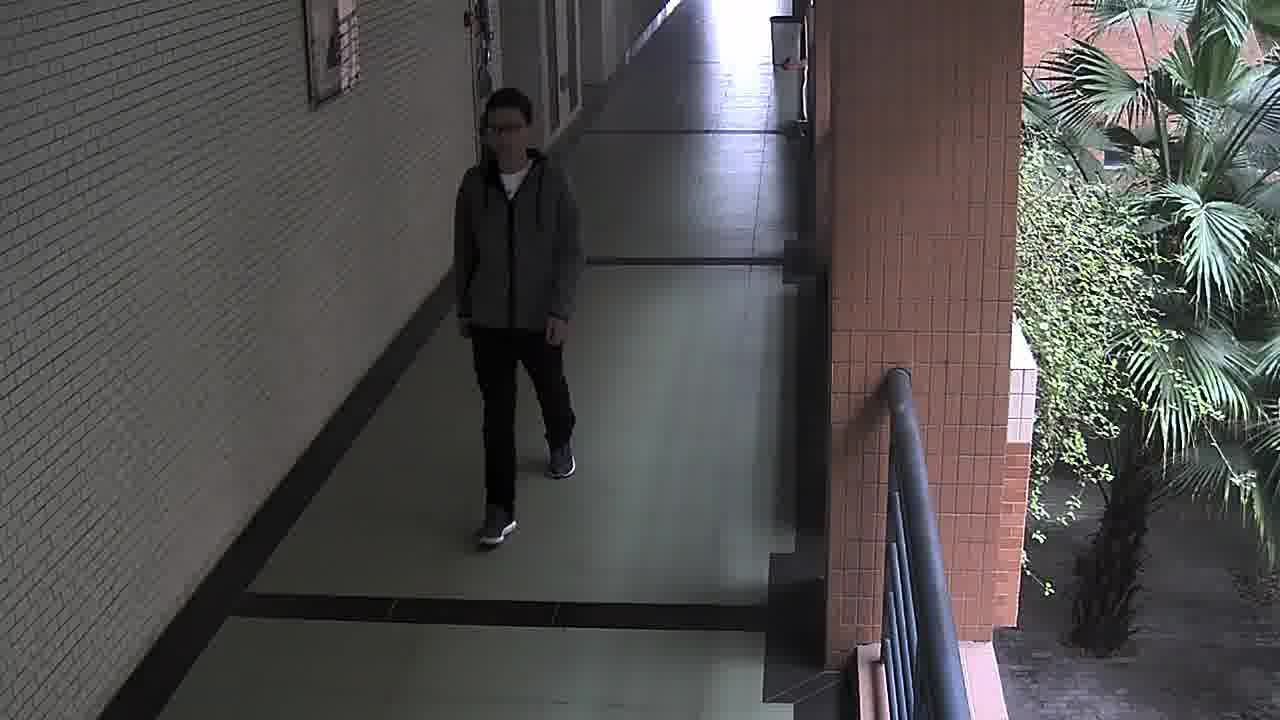
\includegraphics[width=12mm]{figures/2-2}~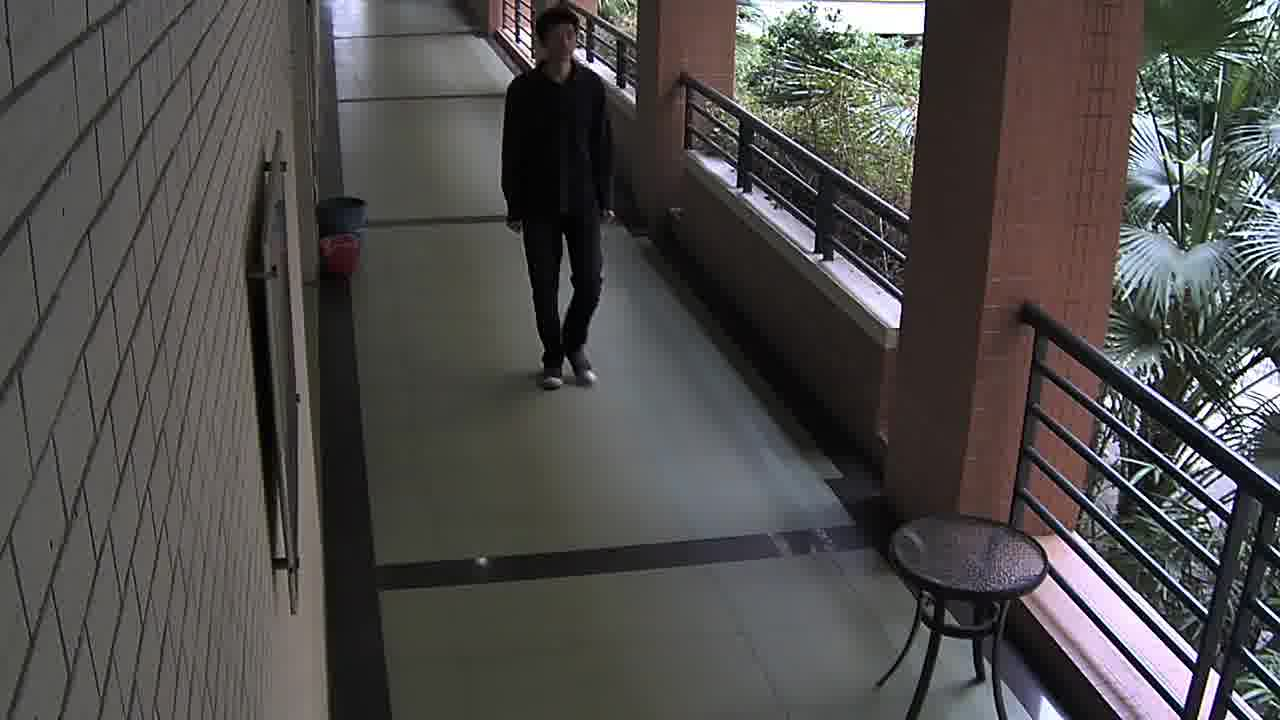
\includegraphics[width=12mm]{figures/2-3}~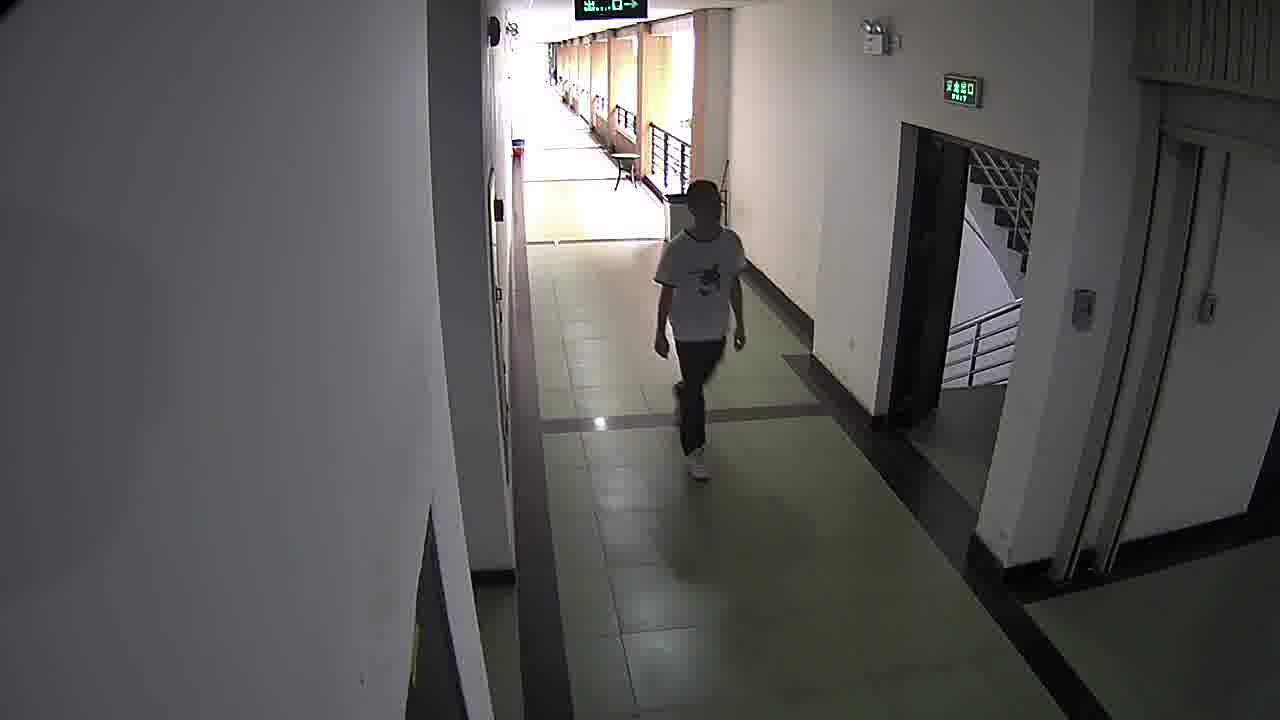
\includegraphics[width=12mm]{figures/2-4} \\
        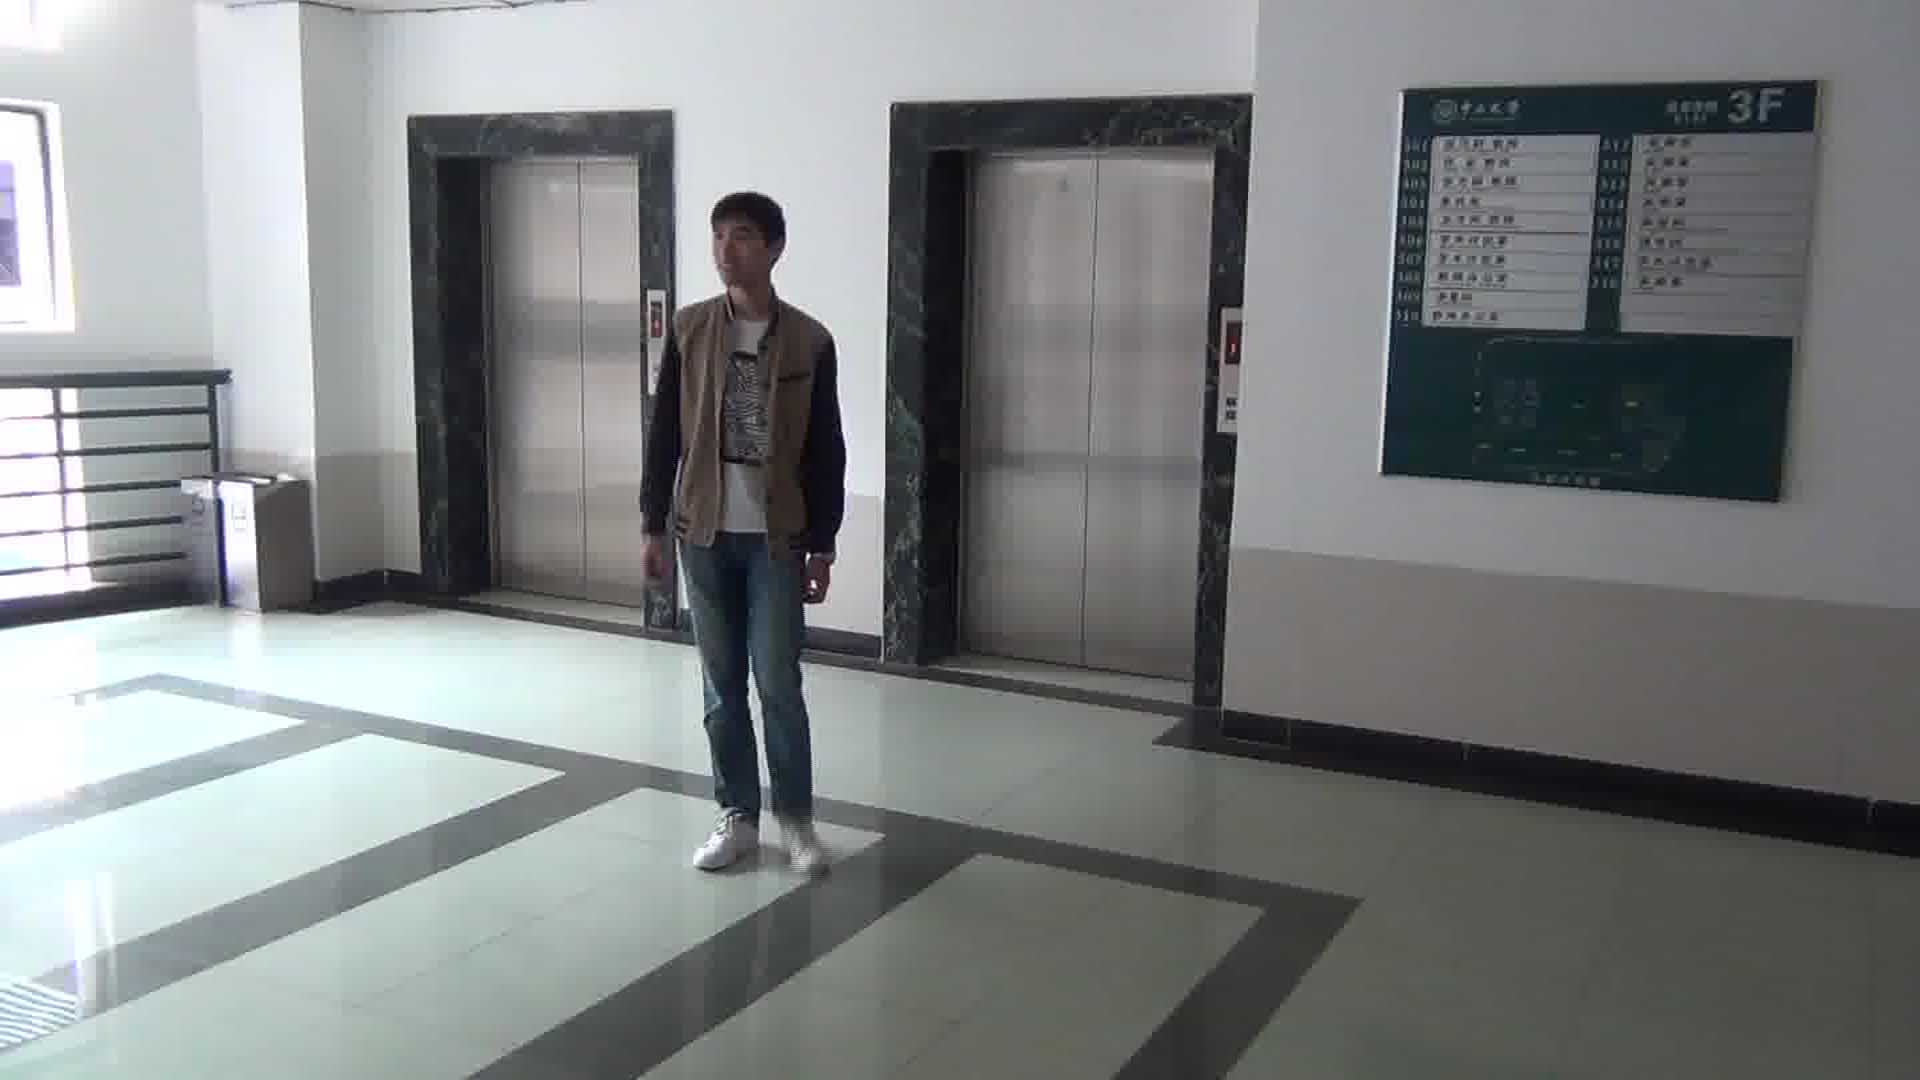
\includegraphics[width=12mm]{figures/3-1}~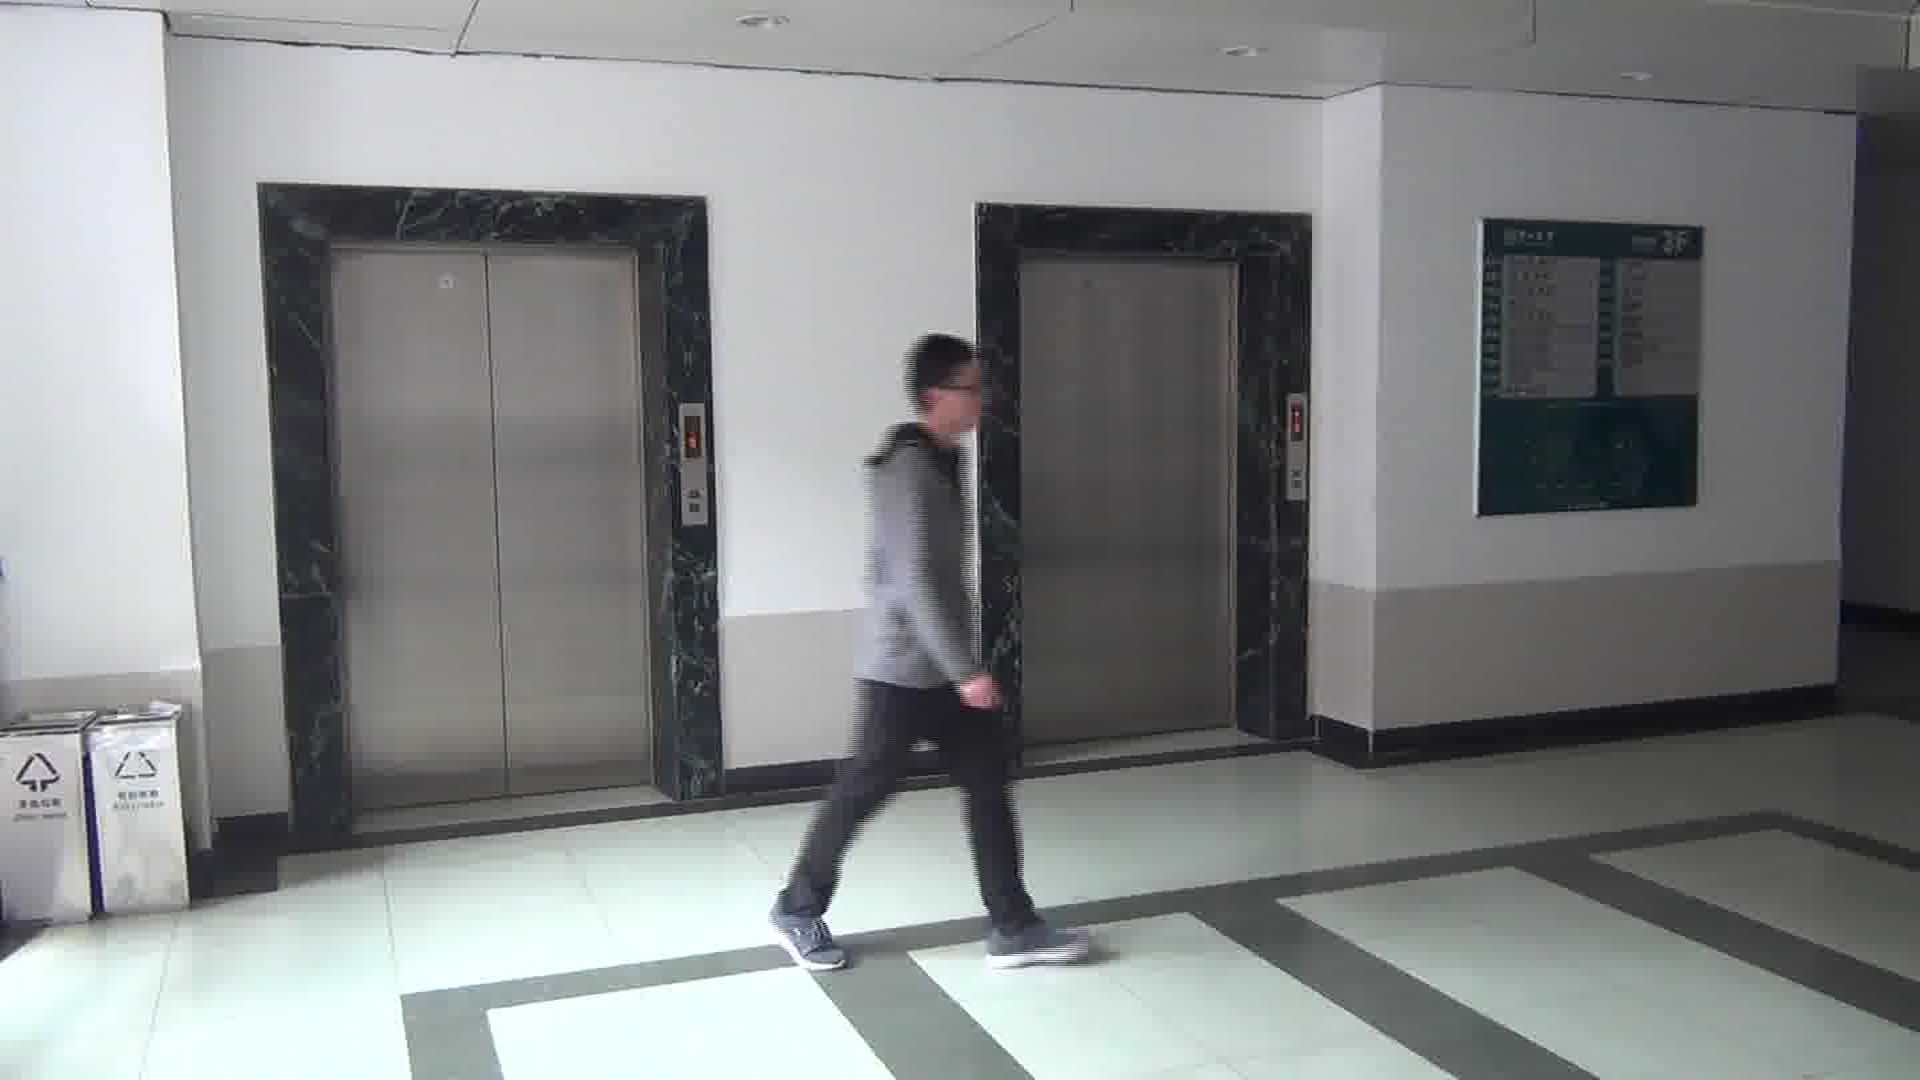
\includegraphics[width=12mm]{figures/3-2}~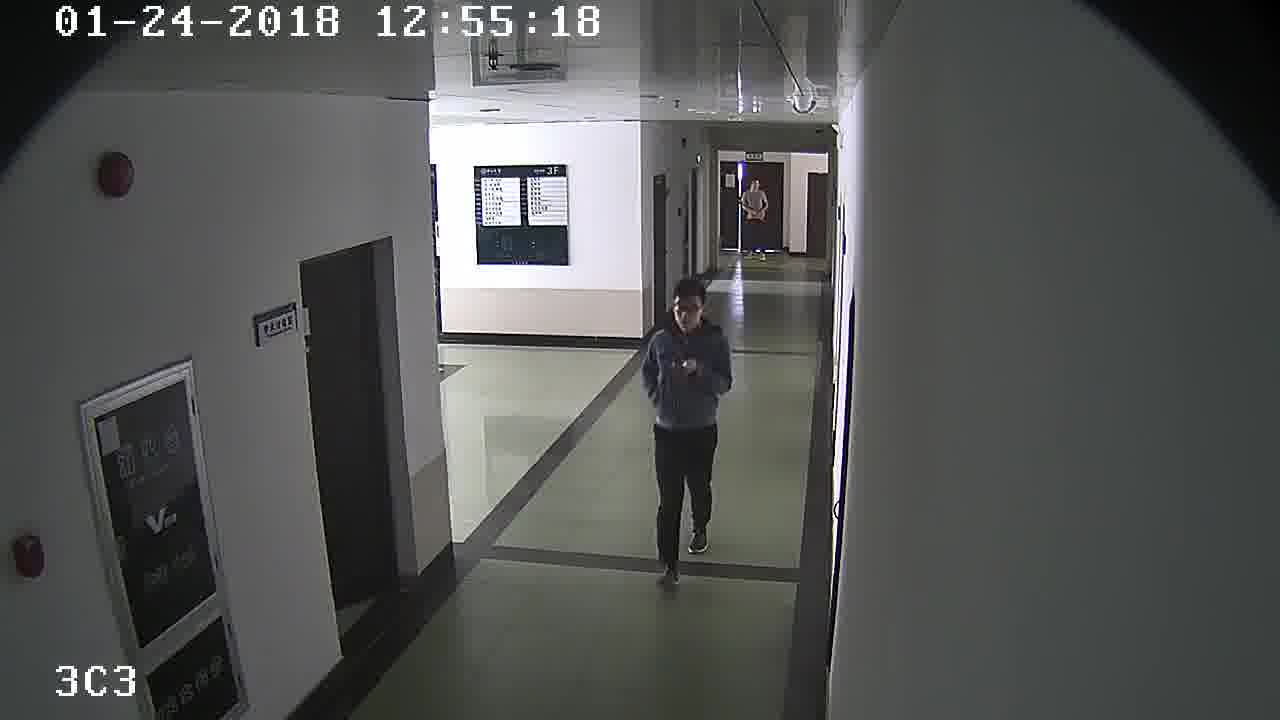
\includegraphics[width=12mm]{figures/3-3} \\
        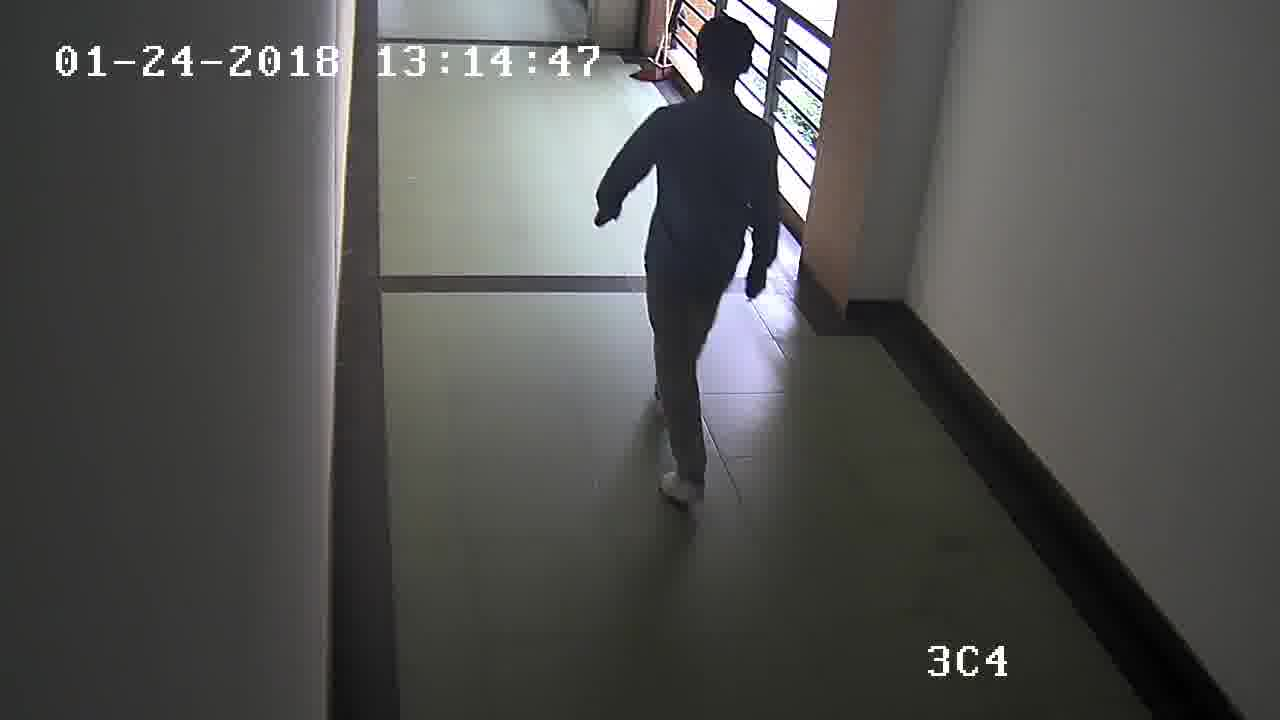
\includegraphics[width=12mm]{figures/3-4}~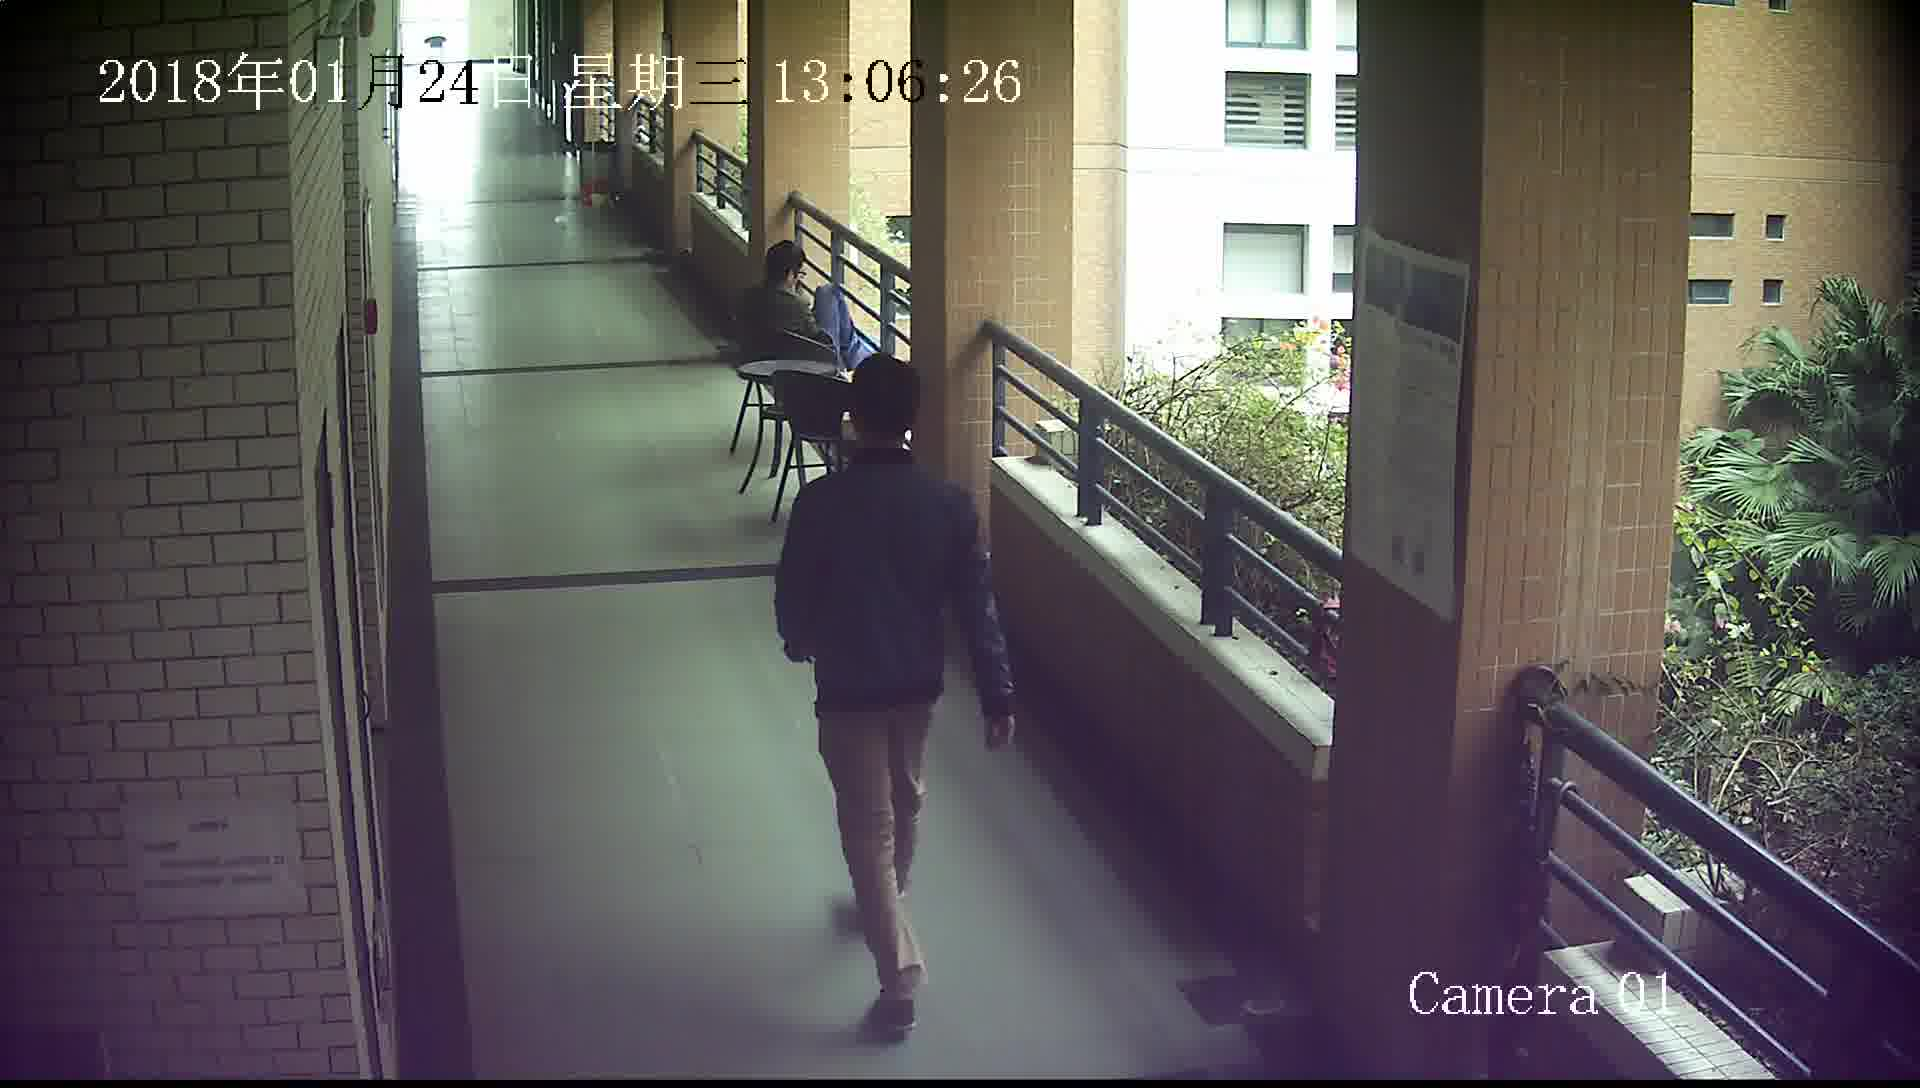
\includegraphics[width=12mm]{figures/3-5}~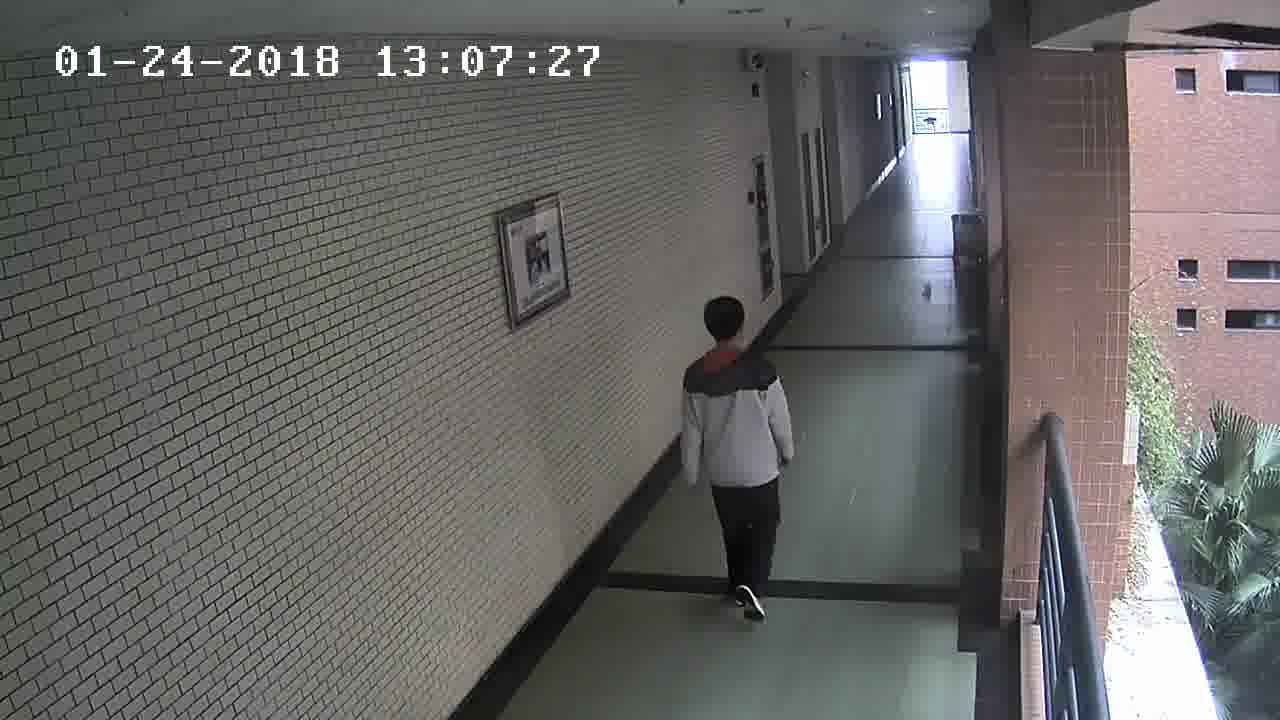
\includegraphics[width=12mm]{figures/3-6}~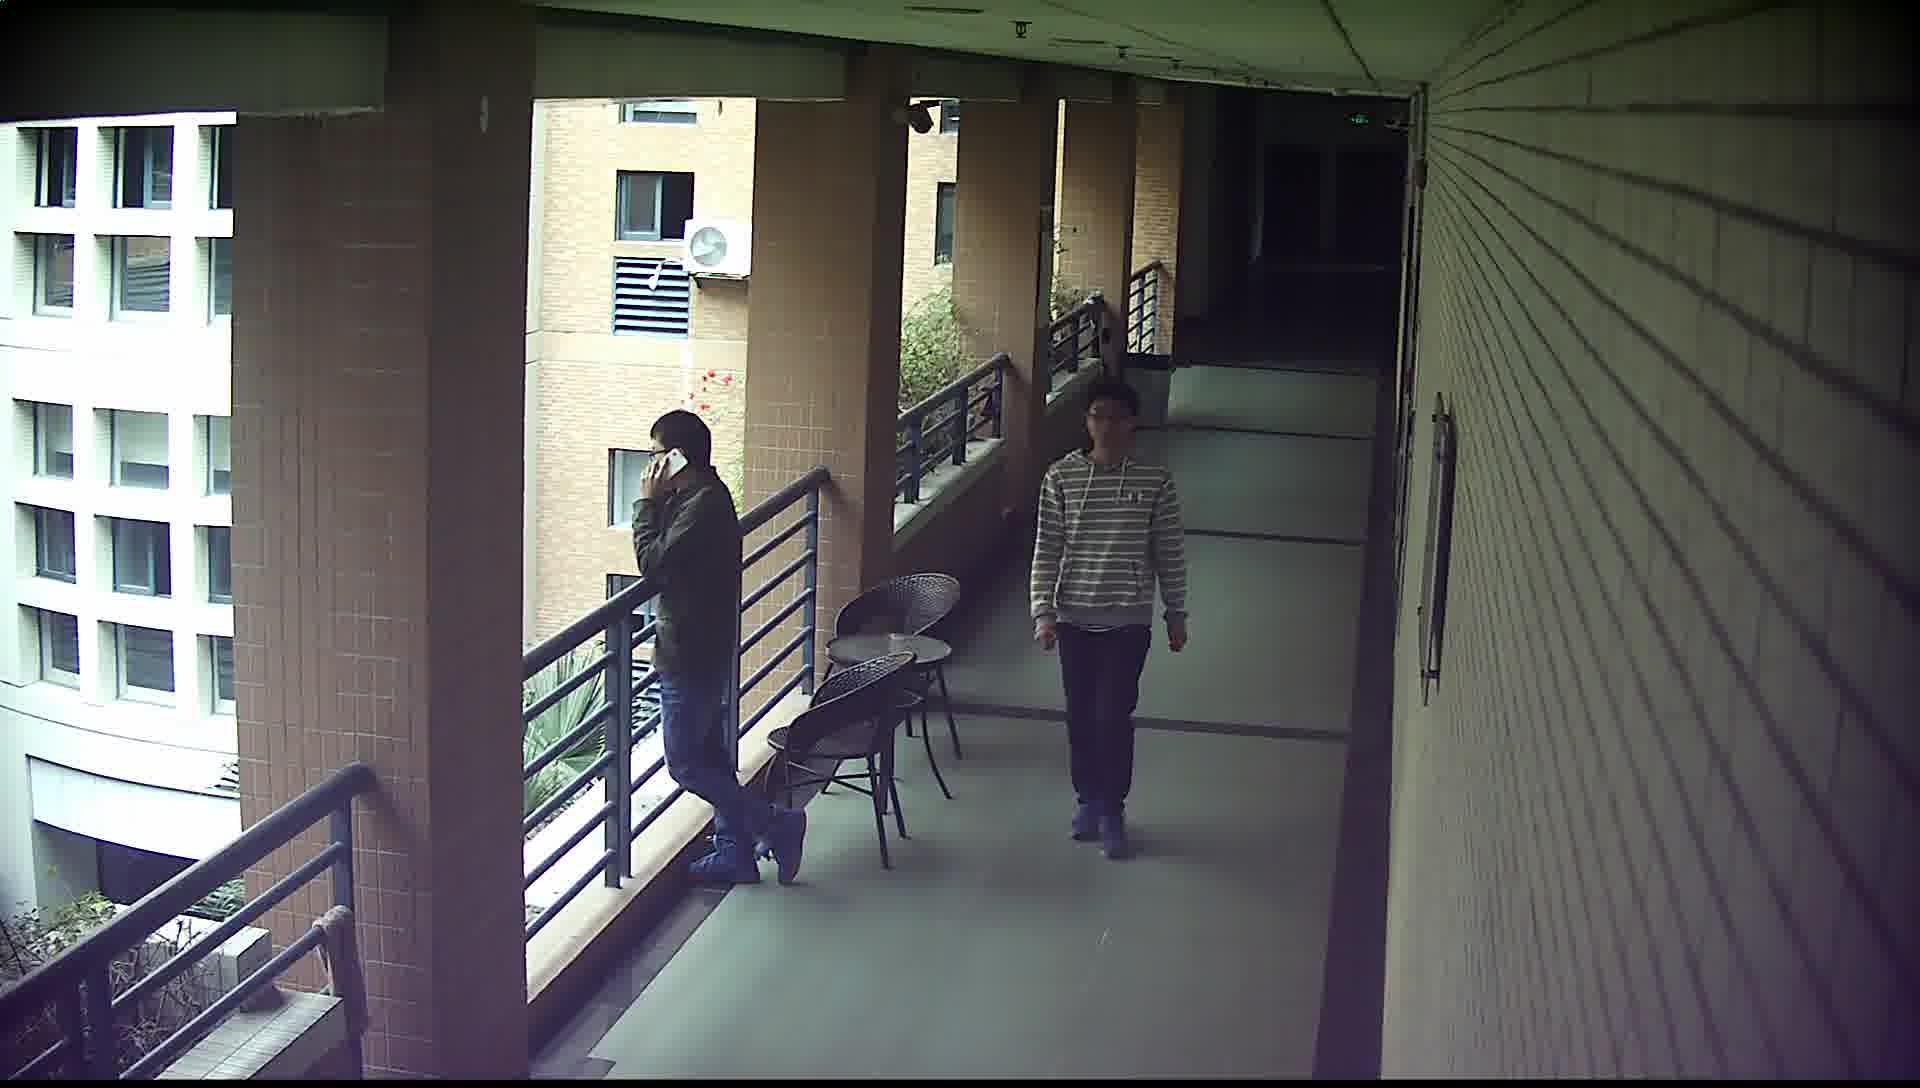
\includegraphics[width=12mm]{figures/3-7} \\
    \end{tabular}
\end{table}
\end{frame}


\begin{frame}{多集群CPU}
\begin{block}{}
    目前大部分深度学习模型都是借助GPU来调整模型参数。\\
    \vskip 1em
    \textbf{GPU 缺点:}
    \vskip 0.5em
    \begin{enumerate}
        \item GPU设备通常比较昂贵,且少见于嵌入式设备中\\[0.5em]
        \item GPU的显存普遍不高,限制了模型的规模及数据量
    \end{enumerate}
    \vskip 1em
    \textbf{多CPU集群优势:}
    \vskip 0.5em
    \begin{enumerate}
        \item 硬件成本低、搭建方式灵活以及部署广泛\\[0.5em]
        \item 对于深度学习算法在多CPU集群上的研究与应用少之又少
    \end{enumerate}
\end{block}
\end{frame}

\subsection{主要工作}

\begin{frame}{主要工作}
\begin{block}{}
    \begin{enumerate}
        \item 实现了行人重识别领域最新的研究成果;\\[1em]
        \item 推出了一个全新的、包含多个摄像头的数据集的初始版本;\\[1em]
        \item 提出了基于强化学习的摄像头部署方案选择模型;\\[1em]
        \item 展示了将模型部署在多 CPU 集群上训练的结果。
    \end{enumerate}
\end{block}
\end{frame}
